\documentclass[11.5pt, oneside]{article}   	% use "amsart" instead of "article" for AMSLaTeX format
\usepackage{geometry}                		% See geometry.pdf to learn the layout options. There are lots.
\geometry{letterpaper}                   		% ... or a4paper or a5paper or ... 
\geometry{legalpaper, portrait, margin=1in}
\usepackage[parfill]{parskip}    			% Activate to begin paragraphs with an empty line rather than an indent
\usepackage{graphicx}				% Use pdf, png, jpg, or eps§ with pdflatex; use eps in DVI mode
\usepackage{amssymb}
\usepackage{multicol}
\usepackage{abstract} 
\usepackage{graphicx}
\usepackage{caption}

\title{Saito: A Big-Data Blockchain with Proof-of-Transactions}
\author{David Lancashire}
\date{October 1, 2019\\v. 3.0.0}
\begin{document}
\maketitle



\begin{onecolabstract}
Saito is a blockchain designed to process terabytes of data every day. The network scales by using a consensus mechanism that turns the collection of fees and the routing of transactions into the major form of work rewarded by the network, and by using a pruning method that lets market forces rather than developers control the amount of data that is stored on the blockchain. Saito continually evolves towards an optimal network structure while eliminating sibyl-attacks, fee-recycling attacks, block-withholding attacks. It offers a decentralized and efficient platform on which to build bandwidth-intensive Internet applications like email, social networks, cryptocurrency payment channels, and much more.
\end{onecolabstract}


\begin{multicols}{2}
Saito is a cryptocurrency designed for applications that need to send large amounts of data across the Internet. The design corrects all known economic problems that exist in conventional blockchain designs, permitting scalability to the point that underlying network hardware rather than economic limitations impose constraints on blocksize. We believe the practical limit for a Saito blockchain today is on the order of 100 TB of data per day, and advances in routing capacity will push us to the petabyte level within a decade.

In the next section we describe the two major problems with all non-Saito blockchain mechanisms.

1. THE ECONOMIC PROBLEMS

The limits to blockchain scaling do not exist at the network technology layer. At time of writing, data centers around the world are implementing 400 Gbps network switches while 100 Gbps connections are becoming standard even in lower-tier colocation facilities. If blockchains could pay for high-throughput equipment it would be easy to build scalable networks.

The problem is that blockchains do not pay for such equipment, instead paying for "mining" and "staking" as these are forms of work which can be objectively measured in a decentralized network. Agreement throughout the network on who is doing work is critical as these networks use such work to regulate who has the right to produce blocks, and thus collect payments. The restriction of payments to miners and stakers is made to protect the system, with the expectation that those miners and stakers who receive payment will pay for whatever the network needs.

But this is where one of the major problem lie: for the fact that miners and stakers are getting paid for mining and staking does not mean they have an incentive to pay for other kinds of activities that are needed by the network. Putting time and effort into unpaid activities like servicing users, collecting transaction fees, or storing data for users and supporting lite-clients is strictly unprofitable. And so miners and stakers refrain from these activities. This is not be crippling at small scale, but as a blockchain grows the costs of these unpaid activities becomes increasingly severe.

The incentive that nodes have to focus disproportionately on paid activities instead of those activities which produce greater value for the network is known in economics as the "free-rider" problem. This is one of the most common types of collective action problems and market failures.

A second problem with blockchain incentives involves the requirement that the added to the blockchain must be maintained in perpetuity. Adding data is profitable for the node that does it, but leads to bloated blockchains that eventually collapse. Satoshi's solution may be "not to care," but indifference to the costs of data storage is not a viable option in high-throughput networks.

In economics these two problems are known as collective action problems. The "free-rider" problem describes the incentive that miners and stakers have to focus only on paid activities and pass all other costs to other nodes in the network. The problem with blockchain creep is a variation of the "tragedy of the commons". These problems emerge because the incentives are broken at the lowest level in POW and POS networks: people are getting paid for activities that do not contribute value to the network.

Fixing blockchain requires solving these two problems: we must pay for routing activities instead of unrelated activities like mining and staking. And we must develop a way for the market (not developers!) to determine how much it costs to keep data on-chain, and prevent nodes from collecting money today for work that others will be forced to do in the future.

2. PAYING FOR ROUTING

Saito adds cryptographic signatures to the network layer. As unconfirmed transactions are passed into the network, the routing nodes add signatures to them that indicate to whom they are being relayed. This makes it possible to develop a measure of "routing work" provided by the nodes in the network.

When a node in a Saito-class network wishes to produce a block, it examines whether the transactions in its mempool contain enough "routing work" to meet the difficulty requirements required to produce a block. The amount of "work" embedded in any transaction is the value of its fee halved by each additional hop beyond the first that the transaction has taken into the network.

Consensus rules specify that nodes cannot use "routing work" from transactions that do not include them on their routing path. In order to incentivize block producers to form if there are not enough of them in the network, we also specify that any surplus value of "routing work" may be taken by the block producer in immediate payment for block production.

One a block is produced, a proof-of-work mining contest then begins to determine who has the right to get paid for it. The challenge is encoded in the block hash. If a miner finds a solution to this challenge it broadcasts it as part of a normal Saito transaction. We call the solution the "golden ticket". If it is included in the very next block produced that activity will trigger the network to issue payments. 

In a basic Saito implementation, the block reward is split between the miner that found the solution and a routing node selected from the transactions included in the previous block. The chance of any routing node winning is made is proportional to the amount of routing work that it contributed to the block. 

Mining difficulty auto-adjusts until the network produces one solution on average per block.






In the Saito network we make two changes to enable terabyte-level scaling. The first is embracing a "transient blockchain" that solves the tragedy-of-the-commons problem inherent in blockchain design, and the second is the use of a novel consensus mechanism that we call proof-of-transactions (a.k.a. proof-of-routing or proof-of-relay) that solves the free-rider problem. 

The principle behind the transient blockchain is simple: allow the nodes in the network to delete the oldest blocks in the ledger at predictable intervals ("genesis periods"). The length of the genesis period can be set dynamically if needed. At the extreme of a blockchain designed to handle global email traffic, it may be as short as 24 hours.

As such, the transient blockchain can be considered a form of pruning where the UTXO slips added to new blocks simply become unspendible after a certain number of blocks, with this limit enforced by the consensus rules of the blockchain: transactions spending outdated slips are invalid by default. With no need to maintain a permanent ledger our transient blockchain makes it possible to accurately predict the true cost of transaction storage, as old transactions are removed at roughly the same rate that new transactions are added.\footnote[1]{The most resilient parasite of an idea in the blockchain community is the rarely-challenged notion that blockchains require permanent ledgers. This is entirely false -- the purpose of a consensus mechanism is to allow the network to reach consensus about which tokens being *added* to the network have value. This value must persist for long enough that the network can fund its own operations. But none of this requires all tokens to have value in perpetuity.}

Under this system, the burden of archiving the network history passes -- as it does in the consumer Internet -- from the routing nodes in the network to the servers and users that actually care about the data. And in cases where it is desirable for data to remain on-chain, it can simply be rebroadcast to the front of the chain with the appropriate fee to cover the next genesis period. The automatic rebroadcasting of expiring slips can even be enabled, if desired, through the consensus rules of the blockchain.

Critics may note the security trade-off in this approach: the idea that new nodes joining the network become vulnerable to attack at their point of initial connection. Yet this is not a problem unique to Saito, as the security that syncing from the genesis block offers is largely illusory. How many Bitcoin users check that their software is syncing from the correct hash? And how can they be sure the software is using that hash? The reality is that security in software packaging and deployment cannot be reduced to a hash, and we must get rid of the illusion that it can to create a truly secure and decentralized Internet.

The transient blockchain avoids the problem of the blockchain growing too large for network nodes to store, and ensures space on the blockchain can be priced accurately even as storage times approach infinity. However, it does not pay for the bandwidth needed by nodes in the peer-to-peer network. To solve this second problem we requires a new security method we call proof-of-transactions:

3. PROOF-OF-TRANSACTIONS

Under proof-of-transactions, any node can create a block at any time provided it pays the cost of a "burn fee" set by the network. This burn fee is set to a high value immediately after a block is found and decreases gradually until it hits zero. Since nodes will issue blocks as soon as it becomes profitable for them to do so, our pace of block production is determined by the overall volume of transactions in the network.

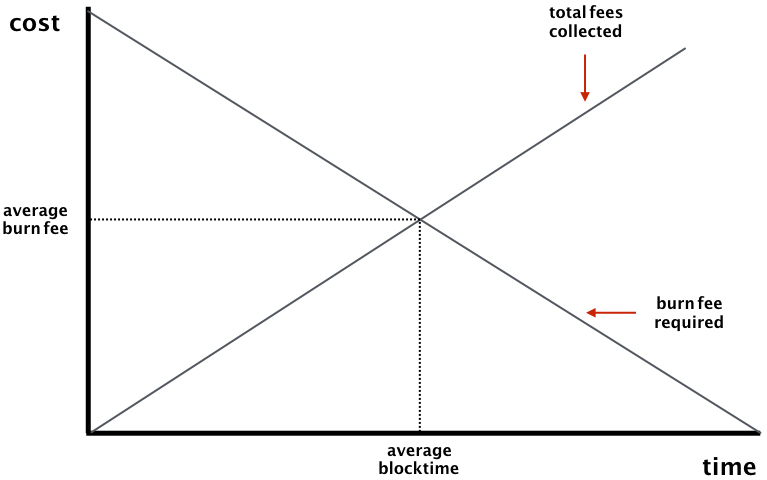
\includegraphics[width=.45\textwidth]{saito2.jpeg}

Our burn fee makes attacking the network expensive, since any increase in the pace of block production requires attackers to pay more in transaction fees than the network is actually collecting. In practice, this means attackers must burn their own capital to attack the network by creating fake transactions that include real fees. It can be easily seen from Figure 2 that it is impossible for attackers to produce blocks at a faster pace than the main chain without taking this step.

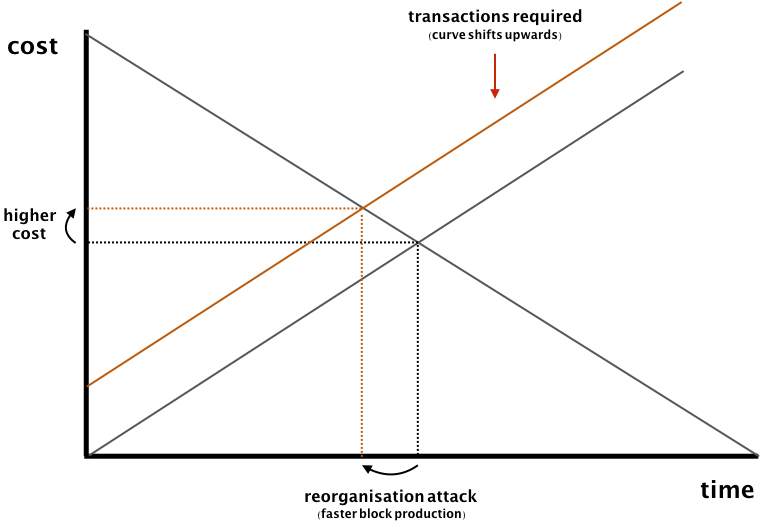
\includegraphics[width=.45\textwidth]{saito3.jpeg}

For reasons that are outlined in Section 4, Saito forces attackers to pay the entire burn fee rather than just cover the marginal difference over the main chain. We also increase the cost of attacks over time by increasing the burn fee to keep blocktime constant as transaction volume grows. This allows the network to offer comparable security to Bitcoin in the sense that the cost of a chain-reorganization attack can always be quantified, and users and applications that require significant guarantees against non-reversibility can calculate the cost of a reorganization attack and wait for the appropriate number of confirmations needed to make chain reorganizations improbable.

There is a major problem with this approach however, which lies in the economic consequences of requiring nodes to burn capital to produce blocks:

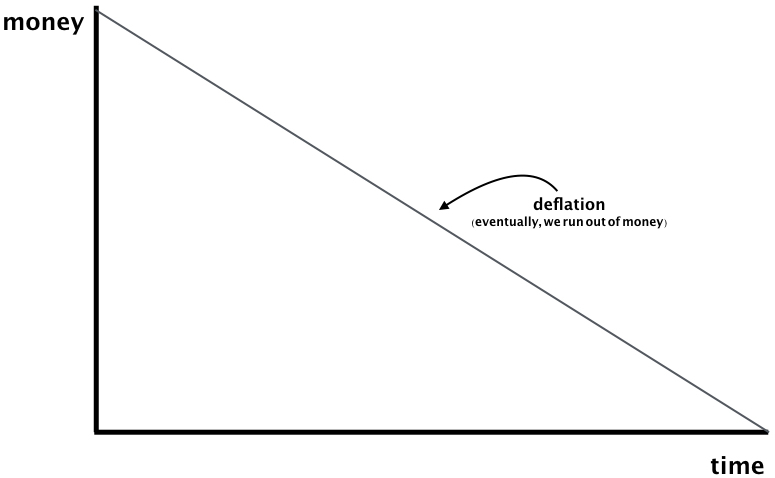
\includegraphics[width=.45\textwidth]{saito4.jpeg}

Avoiding a deflationary crash requires us to inject tokens into our network to keep it from collapsing. Saito's implementation cannot follow in the footsteps of Bitcoin, which solves this problem by attaching the coinbase directly to blocks. To do so would eliminate the entire point of having a burn fee as there is no point in spending money to produce a block if one is immediately reimbursed. As long as block-producing nodes have any influence over how funds are allocated a savvy attacker can sibyl the network for profit, earning profits less by processing transactions and more by gaming the token-issuing mechanism.

Fortunately, there is a solution to this problem, which involves the recycling of the burn fee back into the network through a process that cannot be coopted by any of the players in the network. We achieve this through a zero-sum competition between bandwidth-expending nodes and CPU-expending miners in the network. We call this battle for the "paysplit" of the network.

4. PAYSPLIT

Whenever a node produces a block, it collects what profit it can and bundles all remaining fees into a "golden ticket" that contains (1) a computational puzzle for miners to solve, and (2) a vote to increase, decrease, or hold constant the "paysplit" of the network (the percentage of all golden tickets that are paid out to miners). By default, these tickets are included in all blocks produced. Miners listening on the network then choose which blocks to solve and -- should they find a solution to the cryptographic puzzle -- propagate their solution back into the network as a regular fee-paying transaction. In addition to a proof-of-solution, these miner transactions also include a separate vote on whether to increase, decrease, or hold constant the difficulty of the computational puzzle.

The golden ticket system can be visualized as follows:

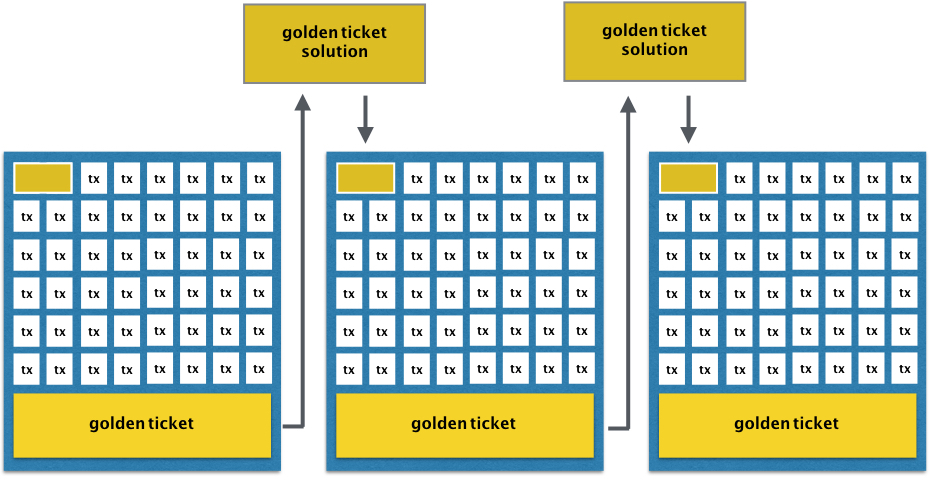
\includegraphics[width=.45\textwidth]{saito7.jpeg}

In order to increase the security of the blockchain, we specify that only one solution may be provided for any golden ticket, and that solution must be included in the very next block. If these conditions are met, our two votes take effect, and the funds locked into the golden ticket are released to the network, split between the miner that found the solution and a random node in the peer-to-peer network. In the event a "golden ticket" is not solved, the funds are locked away and eventually fall off the transient blockchain, at which point they can be recycled back into our economy in the coinbase of another golden ticket. 

This game is counterintuitive to most bitcoiners because it separates the act of "producing blocks" from the act of "issuing tokens". This puts all actors into a delicate dance requiring collusion and cooperation alike. While both nodes and miners want at least one solution per golden ticket (because otherwise no-one gets paid), their interests otherwise diverge: miners prefer a high paysplit and high difficulty level, while nodes prefer a low paysplit and low difficulty level. Given that votes must pass between both players to change consensus settings, we end up with a competitive dynamic where agents in both groups are constantly trading-off their individual short-term against their collective long-term interests.

There are many obvious variants, such as the replacement of a mining puzzle with a proof-of-stake variant. There is also a lite-version of Saito that does not include the voting mechanism at all -- paysplit can be hard-coded so that it can only be changed through a hard fork. Regardless, the key observation on the voting variant is that full-nodes that have miner support will produce blocks at a faster rate and be more profitable than those which do not. Miners who have the support of full-nodes will also be more profitable through negotiating a larger percentage of the paysplit. This creates a dynamic where excessive profits in any sector of the network (i.e. bandwidth provision) will attract competition that will support out-group actors in order to earn immediate supra-market profits. 

The strategies of collusion and defection are determined by the market structure surrounding the economics of bandwidth and security provision. This makes the Saito Network a robust economic design that converges towards an equilibrium point in which the security provided is optimal for both nodes and miners. A useful thought experiment is exploring how the security of this two-player system degrades to offer only bitcoin-level security as the paysplit approaches extreme values.
 
Since we acknowledge that this level is arbitrary and may not reflect the needs of the applications on the network, we allow users on the network to tag their transactions with an optimal paysplit vote. Should a user-originated transaction contain such a vote, our system insists that it can only be included in a block which votes in the same direction. Users who choose to take sides in the ongoing struggle between nodes and miners thus sacrifice the reliability and speed of transaction confirmation, but gain marginal influence over how the network allocates fees.

5. ADDITIONAL SECURITY

Saito takes additional steps to secure the network. In order to deter sibylling,  nodes sign transactions as they propagate through the network, adding to each an unforgeable history of the path it takes from its point of origin to its point of confirmation. Each hop a transaction takes along the network decreases the amount of the transaction fee that nodes can allocate to paying their burn fee, and it's specified that nodes cannot pay burn fees from transactions that do not include them in their transaction path. In order to ensure that nodes cannot influence the distribution of funds from the golden ticket, we also specify that the node in the peer-to-peer network which wins the node share of the golden ticket is selected using a random variable sourced from the miner solution, with the winner selected from the pool of nodes contained in the transaction propagation paths found in the previous block.

These additional restrictions secure our network from common attacks in other cryptosystems which -- oddly -- are not commonly recognized as attacks. In Saito, for instance, transactions are naturally valuable to nodes which participate in the P2P network and useless to attackers who lurk on the edges. Fee-sourcing attacks and transaction theft are also impossible: the fact that nodes must participate in the P2P network to harvest transactions defends us against subtle attacks like those posed by the bitcoin FIBRE network, a closed-access network which benefits its participants by undermining the profitability of nodes which support the peer-to-peer network. Sibylling becomes an unprofitable strategy because it necessarily adds hops in transaction routes, making sibyls visible to other nodes and providing an evolutionary mechanism whereby weaker nodes that permit themselves to be sibylled lose revenue over time. 

This design has the additional benefit of disincentivizing hoarding because nodes that merely participate in transaction routing have a chance of winning the golden ticket reward. Over the mid-term, Saito rewards lite-nodes in proportion to their work as much as it does core network nodes.

Security is also reinforced by the competitive economic structure of our game in fascinating ways. Note that if network security falls too low, the network is incentivized to increase it by voting to pay miners more. How this secures the network is not obvious, but in actuality greater pay for miners increases the amount needed to attack the network. A higher paysplit also supports the threatened chain in the long-run, and speeds up block-issurance as miners compete to have their solutions included over those of their peers. Even in situations where the network is not under active attack, the miner/node battle over the paysplit vote also serves a defensive "canary in the coalmine" function, encouraging miners to issue their own pro-miner blocks if they control enough hashpower to support the block.

6. SUMMARY

Saito is a solution for building a massively-scalable blockchain. We achieve this scalability not through algorithmic tweaks to existing technologies, but rather by solving the underlying economic problems that create distorted economic incentives in all existing blockchain designs.

Those who pour over the technical details of our consensus mechanism will find embedded in it at least seven major innovations in blockchain technology: the transient blockchain, the burn fee, the usable transaction fee, the golden ticket system, the secure multi-party voting mechanism enforced by economic competition, automatic transaction rebroadcasting, and the chain of cryptographic signatures we embed in transactions that permits our network to identify and reward productive nodes in the network.  

We are keen for people to start building on Saito and welcome contact from other blockchain projects looking to incorporate one or several of these methods in their own networks. We have secured provisional patent protection and welcome the creation of a defensive alliance that allows us to share our own knowledge while ensuring that the technologies developed to build big-data applications cannot be perverted to undermine the free-speech values of the blockchain community.

We also encourage everyone to visit our website (http://saito.tech), where we maintain a working demo of the network, a roadmap outlining our development plans, links to downloadable software, and tutorials that can help anyone get started building Saito applications *today*. 

\end{multicols} 
\end{document}
